%Charley Major comments
% Learn how to build clear arguments (discuss in skype call)
% Don't frame the BMT as the option learning model
% No need to treat the KF and BMT as separate models. BMT is just KF when innovation variance = 0

%Charley Minor comments
%Gittins index needs more work

\chapter{Basic Concepts of the Exploration-Exploitation Dilemma} \label{ch:explo}
So far we have seen that there are lots of ideas, concepts and theories about how to solve our coffee shop problem. In this chapter I will describe the basic principles of these ideas (e.g the learning models and the exploration strategies). 

I will begin with a more thorough description of our coffee example as a multi-armed bandit, an experimental design to study the exploration-exploitation dilemma (which is the dilemma that describes our coffee problem). I will explain why optimal decision strategies are intractable and therefore not available for this dilemma. Without the access to those strategies, we need to find alternative solutions.

One such solution is to look at human behavior. We have seen in Chapter one that animals and therefore humans too use trial and error learning. Applied to our coffee example this means testing a coffee shop and learning the outcome. It is not enough to just learn the associations in order to make a decision or to actually solve our coffee shop problem. 
However, we have seen how Rescorla and Wagner used human behavior to model blocking in classical conditioning \citep{rescorla1972theory}, which uses a prediction error as its basis of learning. This showed a shift from merely passive learning to an active learning by making predictions and updating (learning) based on the error between the predicted outcome and the real outcome. 
On this account, we do not only see that modelling human behavior can give us a better understanding of the processes used and help us solve the problem but also gives us a starting point, which are learning models. We need those, because we have to learn from our previous experiences in order to make better decisions.  
Thus, we will take a look at two different learning models. Both take previous experiences into account and update the beliefs when a new experience is made. 

However, learning alone will not be sufficient to solve this dilemma, since it will just help us to learn but not to decide for an action. What we need are strategies that balance the exploration-exploitation dilemma and which give us probabilistic predictions about the options. These strategies are called sampling strategies or exploration strategies. These strategies calculate their predictions based on the current beliefs. After each decision is made, the learning model updates the beliefs based on the new information. 

% Of course, our goal is to model human behavior, but you don't have a clear argumentation structure that leads here. Are we trying to model human behavior to find better solutions to MAB problems? Of course that is one of the reasons, but not the only one, since humans often perform worse than computational bandit algorithms. Rather, this is an interesting problem framework where we want to understand how humans approach this problem.

%Last but not least, we will have a look at a different kind of learning model types: the process model. In more detail the linear ballistic accumulator, which is a model that is based upon sampling evidence over time until a decision is reached. This model includes reaction time, which the other models cannot include. %commented out for now since we don't have plans to include it
\section{Multi-Armed Bandit Problem}
A multi-armed bandit or \textit{k}-armed bandit is a problem in reinforcement learning, which deals with the exploration-exploitation dilemma in a simplified setting, that means we are looking at a simpler version of our coffee problem, for example reduce the complexity of rating the goodness of the coffee.
The problem is named after the "one-armed bandit", a slot machine in casinos, which might give players a reward after pulling a lever.
\begin{figure}
    \centering
    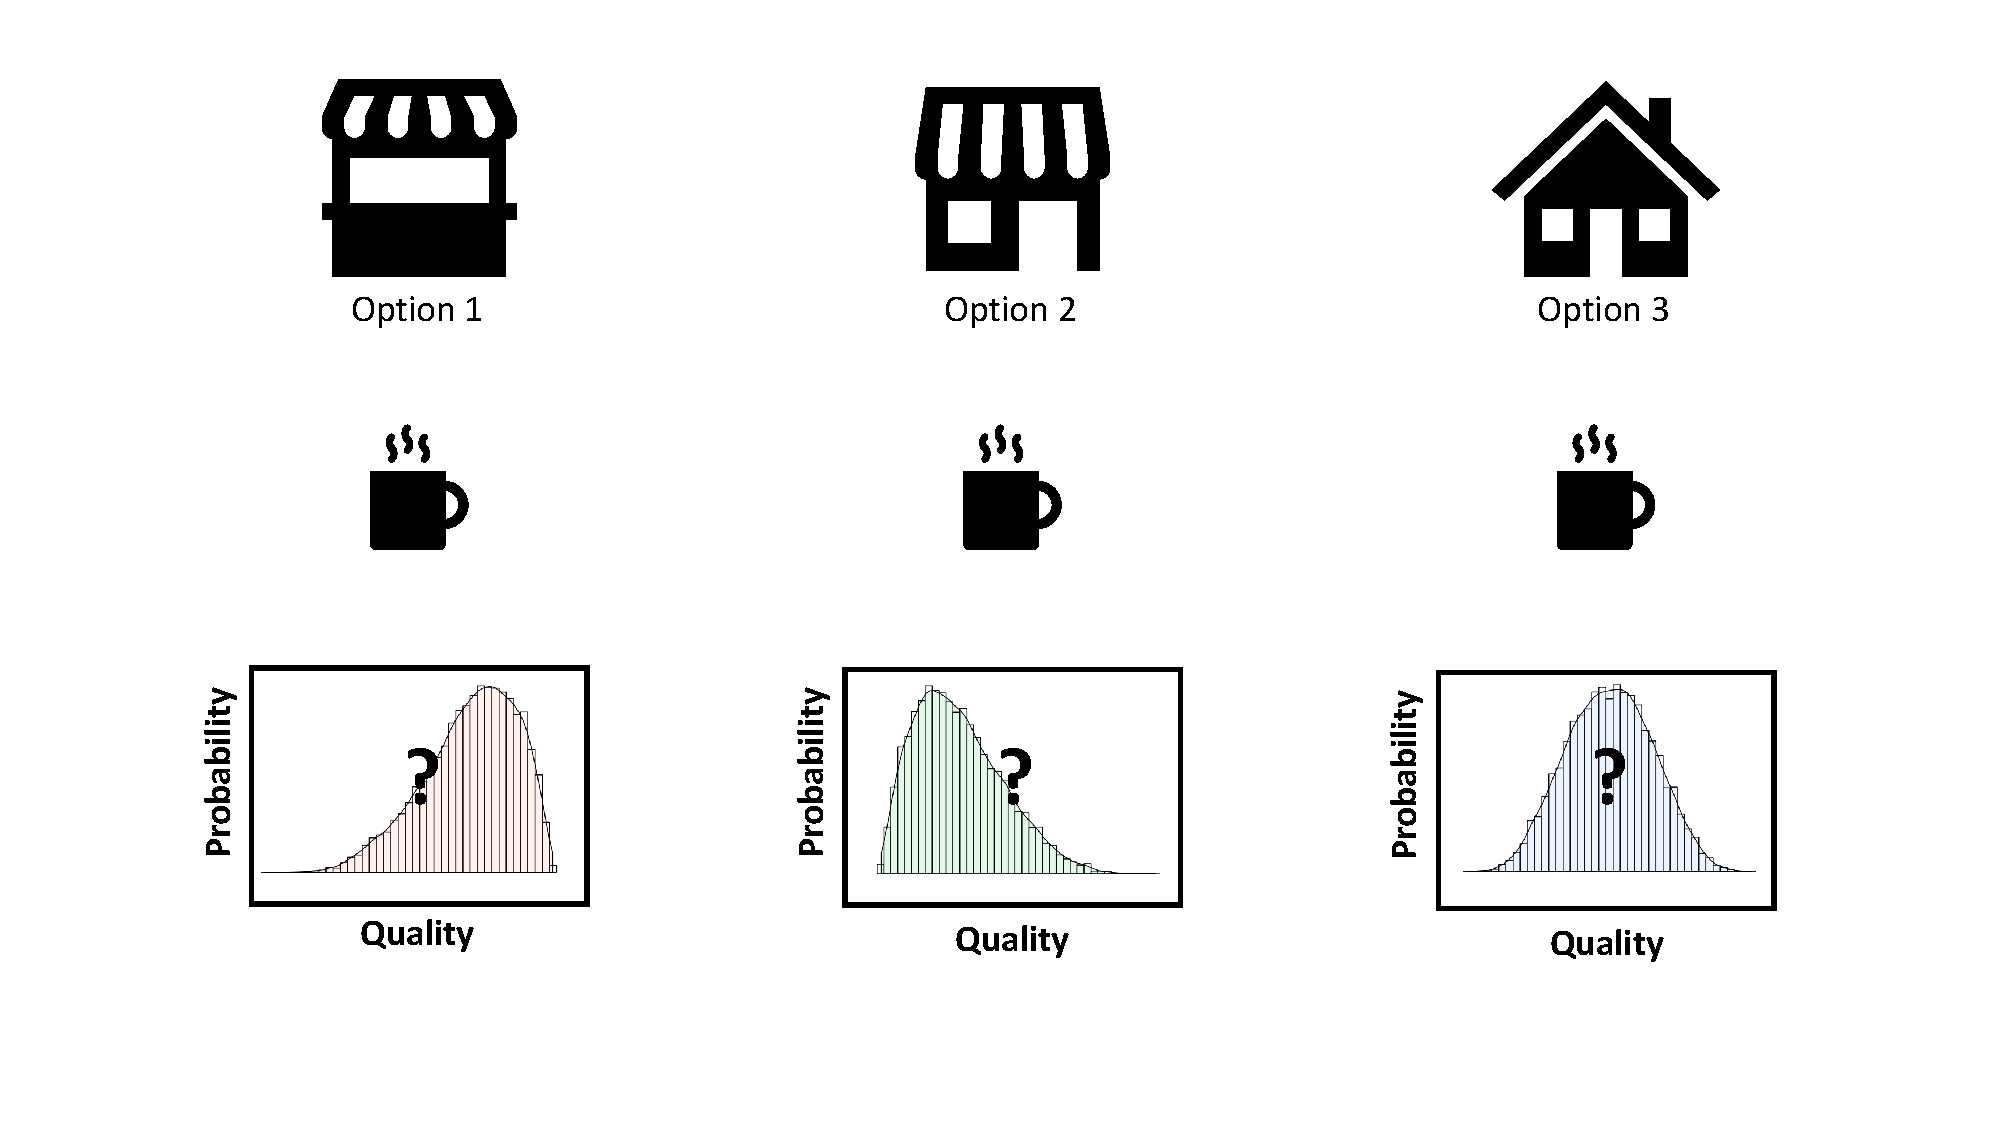
\includegraphics[width=1\textwidth]{Plots/FinalCoffePlot.pdf}
    \vspace{-1.5cm}
    \caption[Bandit Coffee Shop]{A Coffee shop Bandit Problem. Again, we have to choose which coffee shop we want to get the coffee from. Each coffee shop produces coffee with a certain quality and probability, however we do not know the distribution of the probability and quality of the coffee for each shop. However, by exploring, we gain information about each quality and this helps us to figure out the underlying reward distribution. }
    
    \label{fig:CoffeBandit}
\end{figure}{}
The \textit{k}-armed bandit has \textit{k} options, which are called arms, you can imagine those as \textit{k} different slot machines. Choosing an arm (or choosing a slot machine) will give you a numerical reward. 
Typically, the goal is to maximize cumulative rewards over a finite set of actions.

Let's assume that we have knowledge about all rewards for each action, thus we can define a value $q_t(a)$ for each action $a$, which is called the action value \citep{sutton2018reinforcement}: 

\begin{equation}
    q_t(a) \doteq \mathrm{E} [R_t|A_t=a],
\end{equation}
 where $t$ denotes the current timestamp, which is equal to the amount of actions you have already taken plus the current action.
Consider our coffee shop example: You have already chosen a coffee shop four times and are now about to get your fifth coffee, then $t$ would be five. $A_t$ denotes the action that was taken at timestep $t$, while $R_t$ is the corresponding reward. 
%$q_t(a)$ is the value given action $a$ is chosen. 

However, what happens when you do not know everything about all possible rewards? When we do not know what reward we are getting, we have to make some kind of estimation about the action value. We can denote this estimation as $Q_t(a)$. What we have to do in order to solve this problem is to try to get our estimate $Q_t(a)$ as close to the real value of the action $q_t(a)$. Because when we have this as close to the real rewards, we can make better predictions about which action will give us the highest reward in the long run. 
We can only roughly estimate through previous observations what kind of reward will be possible.
To connect this again to the exploration-exploitation dilemma:
choosing an action estimate (e.g. choosing an option you have some information about) is known as exploiting your knowledge; however, if you choose an action with an unknown estimate, this is called exploring. The dilemma now is, do you explore your current knowledge or do you seek out more information in order to be able to make better decisions in the long run? 
The main problem with the bandit is then: how to balance this dilemma? 

\subsection{Optimal solutions}
Optimal solution strategies are usually intractable for the bandit problem, since all possible outcomes for the immediate action have to be taken into account, which can grow exponentially.
Let's consider a two armed bandit where each choice has two possible outcomes. %Note that this is a huge simplification!
Let us return to our coffee shop example, a simple version of the problem, to consider only two different coffee shops, each having binary outcomes of good or bad coffee. This represents the simplest possible bandit problem with two choices and two outcomes. 

One possibility to compute the optimal solution is to consider all possible combinations possibilities and then choose the best combination. This can be represented using a decision tree (Fig.~\ref{fig:DecisionTree}), which will have an exponential number of paths as we increase the problem horizon (i.e., number of sequential choices available). %Devil's advocate. Bandit problems are Markovian, such that the outcome of timestep t depends only on the previous timestep t-1. Thus, you would only have to compute a tree of depth 2
In our current example, we have two options with two possible outcomes for each option. For a horizon of two choices, there are $4^2 (16)$ possible paths (see Figure ~\ref{fig:DecisionTree}). 
Now consider the same bandit for a horizon of 20. This would lead to $4^{20}=1099511627776$ possible paths that need to be considered for only the first decision! In order to make the second decision, we have to calculate the tree again, but with $4^{19}$ possible paths once we have integrated our new information. 
This can grow infinitely and thus is not a computationally possible way to solve the bandit problem, even though it is an optimal solution strategy. %Overall I really like this previous section. However, I'm not sure what you mean specifically when you say "this can grow infinitely". My suggestion would be to switch to continuous rewards to show that the decision tree blows up to infinitely size by only that minor adjustment

Another optimal solution strategy is the Gittins Index. As we have seen, this is also an intractable solution strategy for most bandit problems. It is however, proven to be optimally for stationary bandit problems with a fixed number of options. In other words: the underlying reward functions have fixed probabilities, but are unknown and the number of arms stays the same. The optimal solution strategy for an agent would be to compute the expected total reward for each option at any particular time, which results in the Gittins Index. Then the agent just has to pick the highest Gittens Index. 
This problem is also computationally exponential \citep{gittins1979bandit}, which makes it as the example above impractical. 
As \cite{cohen2007should} pointed out the Gittins Index is intractable for most bandit problems due to its strict assumptions about the environment, especially the assumptions that it needs an infinite horizon in order to be able to compute an optimal solution.  

To sum up, we have seen two possible optimal decision strategies which work in similar ways and we know that both of those are not tractable. Therefore, to solve the bandit problem, we can take a look at how humans solve this problem, which is not with an optimal decision strategy but with a heuristics that performs very near the optimal solution. We call these heuristics exploration strategies. 
\begin{figure}
    \centering
    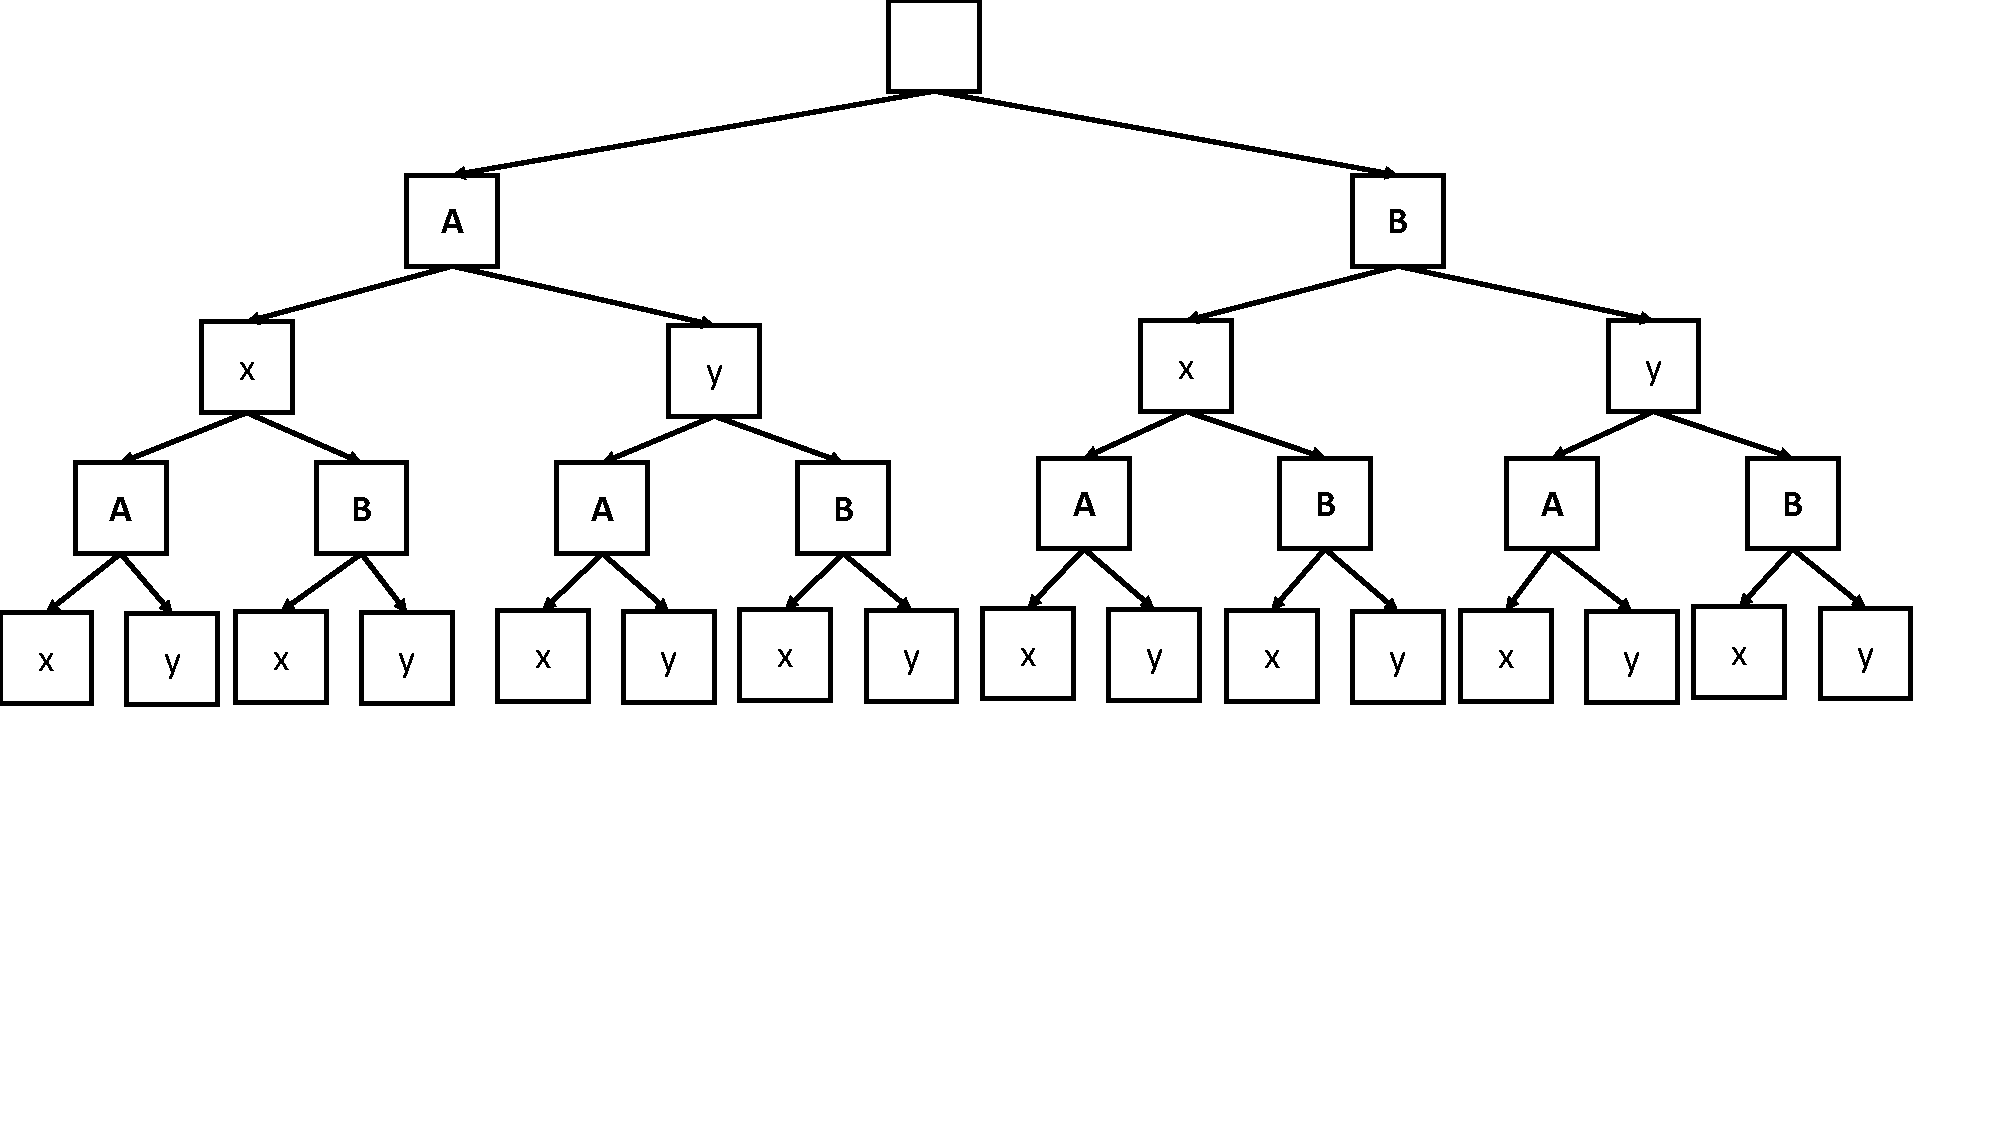
\includegraphics[width=1\textwidth]{Plots/DecisionTree.pdf}
    \vspace{-3.5cm}
    \caption[Decision Tree for Optimal Solution Strategies]{Decision Tree. This shows the decision tree for bandit problem with two choices: A and B. Each choice (A,B) has two possible outcomes (x or y) }
    \label{fig:DecisionTree}
\end{figure}

\section{Modeling human behavior} 
%There are many ways to frame this section, but maybe take the David Marr levels of analysis approach?
Computational solution are not the only way to look at solving the bandit problem. From associative learning, especially classical conditioning, we saw learning models that were able to predict human behavior. The Rescorla-Wagner model was created in order to understand and explain the blocking effect in associative learning. We adapt this approach to understand how humans solve the bandit problem.

By applying a learning model, we have a better understanding of how the learning from one choice to the next can change and how rewards are learned. However, only updating your knowledge is not enough in this task, since it is an exploration task. In order to decide which option to choose and what to learn, we have to explore the options first. Therefore, we need a way to represent exploration; that is where the exploration strategies will come into action. 

In order to model human behavior on the bandit problem, we will not only need a learning model but also an exploration strategy. This combination can then model human behavior and give us a greater understanding how to solve the problem with a good to near perfect solution, since humans do perform really well in these kinds of dilemmas. 

\subsection{Learning Models}
There are many different classes of learning models; they differ in the base assumption on how they work. In our current setting we we will take a look at learning models which are based on Bayesian learning. 
This means, that the models do not learn each association independently but through all trials, each new trial is used to update the belief about the rewards of each option. These beliefs will be used to predict the next outcome, or rather the next action. 

The models are different from the exploration strategies in the sense that they are not build upon the idea to balance the exploration-exploitation dilemma but only to update their beliefs. While the exploration strategies weigh the options in order to choose an action, learning models only work with their previous knowledge; the prior. They update it with the help of the prediction error, which is the difference between the prediction of the model and the actual outcome. Thus the main difference between them is that learning models alone will not tell anything about the exploration, but only about the association. Whereas the exploration models only consider the exploration. Together, they can then form a model that updates the exploration strategies and can therefore imitate human behavior.
We will start to look into a familiar learning model, which is the Kalman Filter, a Bayesian version of the Rescorla-Wagner model \citep{gershman2015unifying}.


\subsubsection{Kalman Filter} %Bayesian version of rescorla-wager
A Kalman filter (KF) is a Bayesian version of the Rescorla-Wagner model \citep{gershman2015unifying} and can be seen as a variant of the delta learning rule. This means that the Kalman Filter works with a prediction error, however it also takes uncertainty of the environment into account. It starts with a model that will estimate the next step, so for example in our coffee case: it will estimate the next coffee shop. Then in the next step the KF updates its previous knowledge and thus the parameters which led to the first prediction, in order to better fit the observed data. It first predicts which coffee shop we would take and then observes what we actually choose and then updates its equation and its parameters in order to give a better prediction the next time around. We assume that the mean $\mu_{j,t}$ for arm $_j$ and trial $_t$, given the previous observations (the arms that were chosen and the rewards) $D_{t-1}$ is normally distributed.
\begin{align}
    p(\mu_{j,t}|\mathcal{D}_{t-1}) &= \mathcal{N}(m_{j,t},v_{j,t})
\end{align}
The mean and variance for the normal distribution are dependent on the previous mean and variance from the trial before. $\delta_{j,t}$ is a variable tracking if the arm we are currently looking at was chosen before. If it is the same arm $\delta_{j,t}$ equals one, zero otherwise. $y_t$ is the observed reward on the current trial. 
\begin{align}
    m_{j,t} &= m_{j,t-1} + \delta_{j,t}G_{j,t}\left[y_t-m_{j,t-1}\right]
    \\
    v_{j,t} &= \left[1 - \delta_{j,t}G_{j,t}\right]\left[v_{j,t-1}+\sigma_\zeta^2 \right]
\end{align}
The Kalman gain $G_{j,t}$, which can be described as the learning rate, weights the chosen arm with the following equation:  
\begin{align}
G_{j,t} &= \frac{v_{j,t-1}+\sigma_\zeta^2}{v_{j,t-1}+ \theta_\epsilon^2+\sigma_\zeta^2}
\end{align}
where $\sigma_\zeta^2$ is the innovation variance, which donates how much the uncertainty grows when an option is not played. The error variance $\theta_\epsilon^2$ includes an inverse sensitivity to the observed rewards, e.g. when it is small, it becomes sensitive to the data and thus will make larger updates for the next trial. However, if the error variance is high, the model does not learn from the trial and barely makes any updates. 
If there was no previous posterior (as it is in the first trial), then a prior set of predictions has to be calculated with the help of the prior variance $\sigma_0$ and the prior mean $m_0$. The prior mean and variance are either estimated or fixed when implementing. In our case we fixed the prior mean to 0 and had the prior variance estimated. Together they define the first mean and variance that has to be updated. 

\subsubsection{Bayesian Mean Tracker} %No need for rewriting all the math again! The BMT is just the KF with innovation variance =0
 
The Bayesian mean tracker (BMT) \citep{speekenbrink2015uncertainty} is a simplified version of the Kalman Filter. In their study, \citeauthor{speekenbrink2015uncertainty}
It is therefore an associative learning model, which will learn the reward distribution of each arm of a bandit problem independently. It differs from the KF in the sense that it only tracks the mean and not the variance with it, i.e. the basic assumption is that the reward remains constant for each arm over trials. 
In our case then, it learns a posterior distribution over the means of each arm. 
This means, that it learns a distribution from which it can estimate the upcoming action value (reward) of an arm. To fit this to our coffee example: it learns how good the coffee from a shop was and can predict how good the next one will be, given the overall goodness of all coffees from this particular shop. We assume that the rewards are normally distributed around an unknown mean but with a known variance. The arms are denoted by $j$ while the mean of a given arm and the trial $t$ is denoted as $\mu_{j,t}$.
\begin{align}
    p(\mu_{j,t}|\mathcal{D}_{t-1}) &= \mathcal{N}(m_{j,t},v_{j,t})
\end{align}
The probability of the mean $\mu_{j,t}$ given the previous observation of all arms $\mathcal{D}_{t-1}$ includes all previous observations until the trial or timestamp t-1, basically every reward that was collected until the point of the next decision. The mean and variance for a certain option are only updated if this arm was selected according to the following equations: 
\begin{align}
    m_{j,t} &= m_{j,t-1} + \delta_{j,t}G_{j,t}\left[y_t-m_{j,t-1}\right]
    \\
    v_{j,t} &= \left[1 - \delta_{j,t}G_{j,t}\right]v_{j,t-1} 
\end{align}
$\delta_j$ will be equal one if arm $_j$ is chosen on the current trial $_t$, it is zero otherwise. $y_t$ is the observed reward and $G_{j,t}$ is defined as: 
\begin{align}
G_{j,t} &= \frac{v_{j,t-1}}{v_{j,t-1}+ \theta_\epsilon^2}
\end{align}
$\theta_\epsilon^2$ denotes the error variance. The probability of the mean of the next choice is calculated by a normal distribution given the previous means and the variance. The variance is known, because all parameters are known and thus the variance can be computed and does not need to be estimated. The mean is calculated and updated by the equation above and is dependent on the previous observed mean, $G_{j,t}$ which normalizes the variance with the error variance, and the previous observed reward subtracted by the previous mean.
\subsection{Exploration Strategies}

%Take $m_j$ and $v_j$ in order to compute a value
\subsubsection{Upper Confidence Bound sampling}
The UCB \citep{auer2002finite} is an example of a directed exploration strategy; it gives an exploration bonus to more uncertain option. This means the more uncertain the option, the higher the probability that it is taken. A weighted sum is used to calculate the value of each option. $m_{j,t}$ is the posterior mean reward of option $_j$ on trial $_t$, while $v_{j,t}$ is the posterior variance of option $_j$ on trial $_t$.
\begin{equation}
UCB_{j,t}=m_{j,t}+(\beta_{\sigma} \cdot  \sqrt{v_{j,t}})
\end{equation}
$\beta_\sigma$ is called an exploration factor. This is the factor that defines how high the uncertainty bonus will be. In this equation we can see that the variance is influenced by the exploration bonus, so that more uncertain options can be picked, even though the posterior mean is not known or low.
\paragraph{Linear Model}
Furthermore, we constructed a version of the UCB, the linear model, which does not only increases the variance by a parameter ($\beta_\sigma$) but also the mean ($\beta_\mu$). 
\begin{equation}
    LM_{j,t}=(\beta_\mu \cdot m_{j,t})+(\beta_{\sigma} \cdot  \sqrt{v_{j,t}})
\end{equation}

\subsubsection{Softmax}
The softmax choice rule is used to convert valuations of choices into a probabilistic choice distribution. In our case, we apply the softmax choice rule after an exploration strategy to make probabilistic predictions about how a human decision-maker will behave. The values will lie in an interval between zero and one, with all four probabilities adding up to one. %Do you really have to tell the reader what a probability distribution is?
For option $j$ on trial $t$, we have the decision value $Q_{j,t}$ upon which we can calculate the probability for the option on the trial. 
\begin{equation}
P(C_{t}=j) = \frac{\exp(Q_{j,t}/\tau)}{\sum_{k=1}^4 \exp(Q_{k,t}/\tau)}.
\end{equation}
$\tau$ is a temperature parameter, which we estimate as a free parameter governing the level of random exploration. %Elaborate on the random exploration intepretation of the temperture parameter
High values for the temperature parameter mean that the probabilities of each option are very similar, while a low temperature value indicates that the option with the highest estimated reward will have the highest probability, which is near 1. 

\subsubsection{Thompson Sampling}
Thompson \citeyear{thompson1933likelihood} sampling is a heuristic strategy for multi-armed bandit problems that is performed by choosing an action that maximizes the expected reward based on a randomly drawn belief. In our setting, we use a form of Thompson sampling that generates $n$ Monte Carlo samples from each option $j$ based on the posterior distribution of action values from the learning models at time $t-1$:
\begin{equation}
    s_{j,i} \sim \mathcal{N}(\mu_{j,t-1},\sigma_{j, t-1}), \text{for } i = 1... n
\end{equation}
Each sample $s_{j,i}$ corresponds to a single sampled belief about the value of option $j$. We then stochastically select an action based on the probability that it is the best option:
\begin{equation}
    P_{C_{t}=j}=\frac{1}{n}\sum_{i=1}^{n} s_{j,i}>s_{k\neq j,i}
    \label{eq:PMU}
\end{equation}
$P_{C_{t}=j}$ denotes the probability of selecting option $j$, which is proportional to the number of times the sampled value $s_{j,i}$ is better than the sampled values of all other options $s_{k\neq j,i}$. This is then averaged over all $n$ Monte Carlo samples.This approach is sometimes also referred to as the Probability of Maximum Utility \citep{speekenbrink2015uncertainty, wu2018generalization}, and exists somewhere in the spectrum between directed and random exploration. Purely random approach would consider each option equally likely and thus have the same probability of being chosen. However, the Thompson Sampling or PMU is still sensitive to the uncertainty and means of each option, since they calculate the probability of each option based on the predictive distribution of either the mean (Thompson) or the rewards (PMU) \citep{schulz2017putting}.

\subsubsection{Hybrid Model}
We also considered a hybrid of Thompson Sampling and UCB, by optimistically inflating the mean of the posterior normal distribution based on the estimated uncertainty:
\begin{equation}
    s_{j,i} \sim \mathcal{N}(\mu_{j,t-1} + \beta\sqrt{\sigma_{j, t-1}},\sigma_{j, t-1}), \text{for } i = 1... n
\end{equation}
This is similar to how the exploration parameter $\beta$ is used in UCB, but here we use the same Monte Carlo sampling technique to generate a set of $n$ sampled beliefs and then compute the choice probability the same as our Thompson sampling model (Eq. \ref{eq:PMU}).




\section{Process models}
Process models are do not only predict the decision but are based on evidence accumulation and therefore also track the reaction time. Evidence accumulation is done over time for each choice until a threshold is reached. When it is reached, an decision is made. The time until enough evidence is accumulated to reach the threshold is equal to the reaction time. The drift diffusion model is one of the most famous models of these kind. 
% \begin{wrapfigure}{r}{0.48\textwidth}
% \begin{center}
%     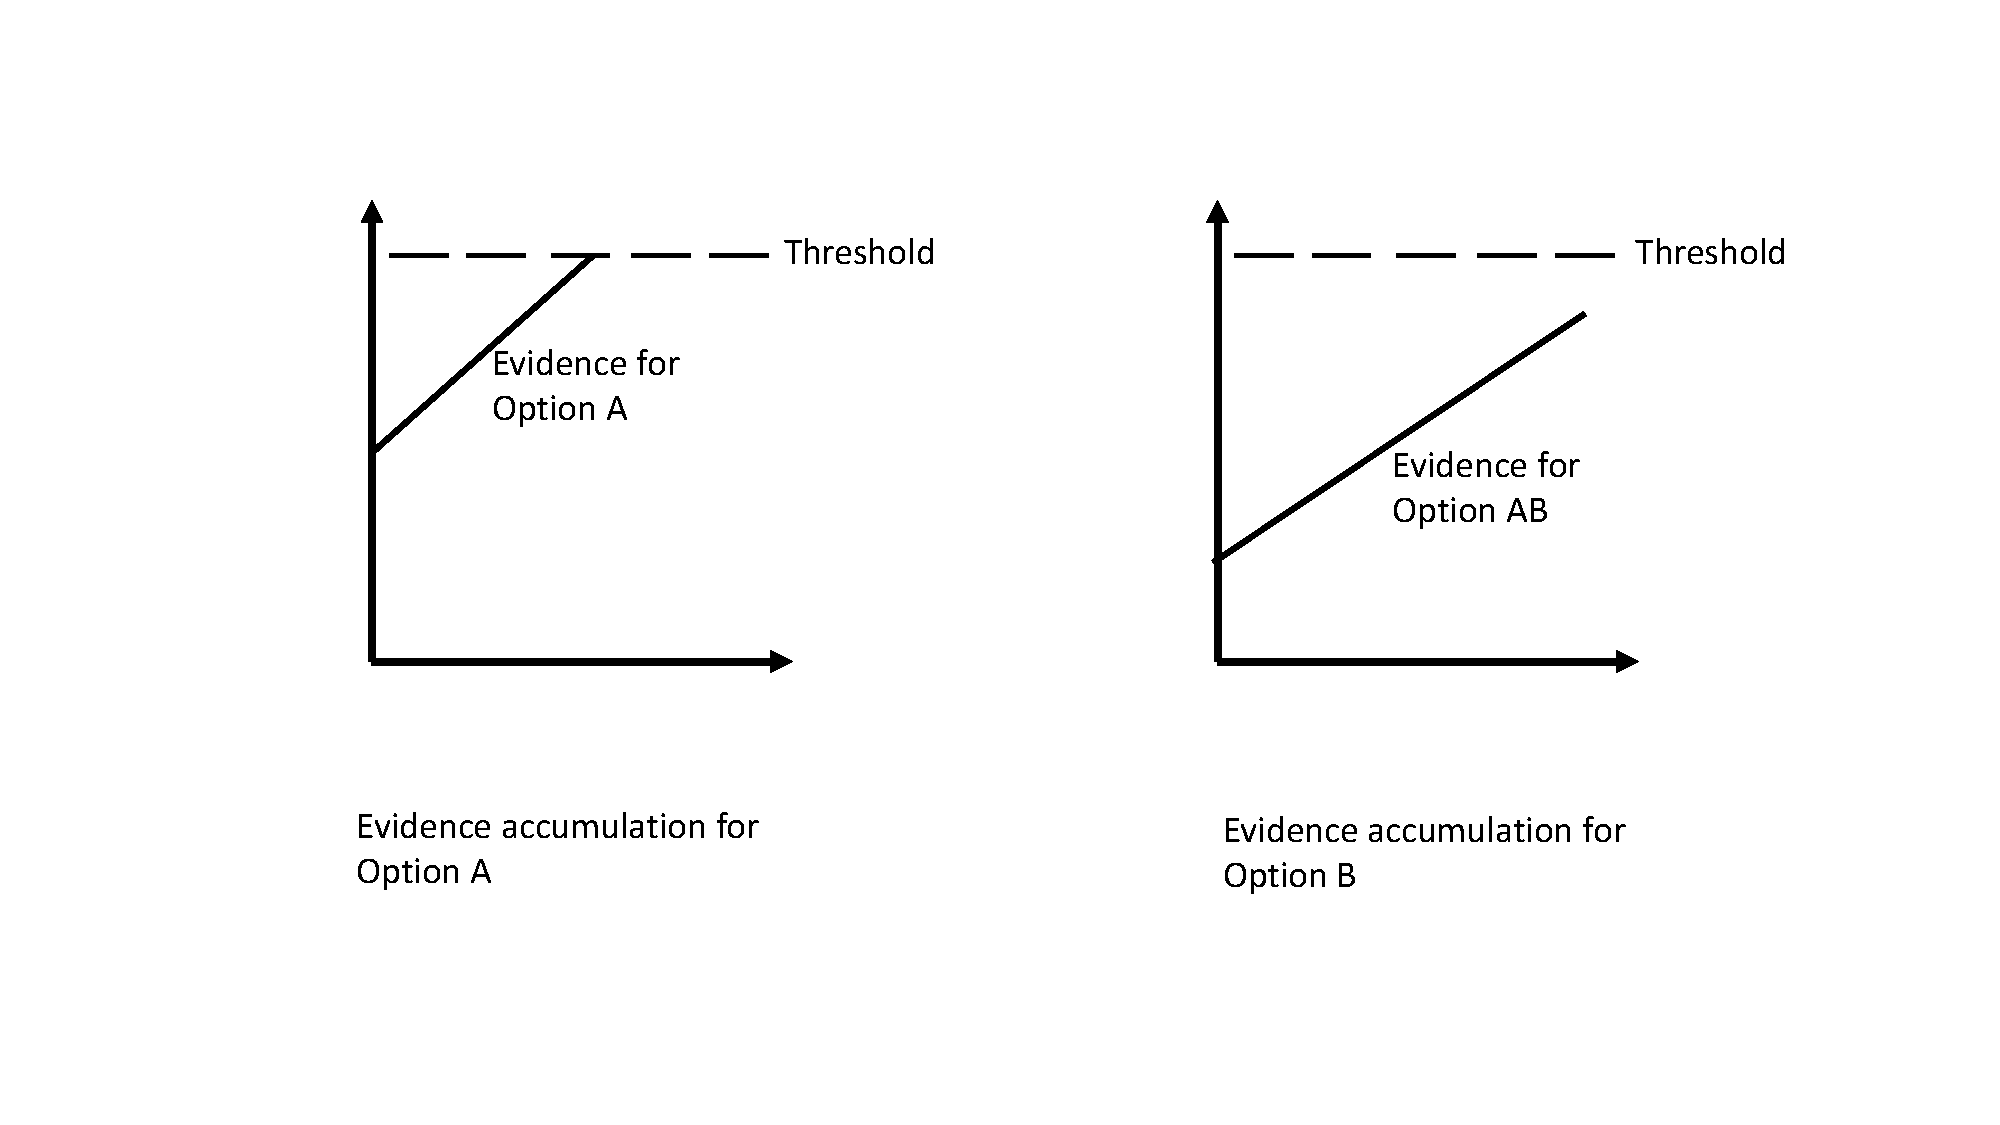
\includegraphics[width=0.6\textwidth]{Plots/LBA.pdf}
% \end{center}
% \caption{}
% \label{fig:LBA}
% \end{wrapfigure}
%Not only predicting choice, but reaction time based on a mechanistic assumption that evidence (for eac a choice) accumulates over time
\subsection{Linear ballistic accumulator}
The linear ballistic accumulator (LBA) models decisions and reaction time. Compared to our other models (KF, BMT), it also models the time needed for a decision. \citep{brown2008simplest} proposes this model as a simpler alternative for the drift diffusion model. For each option (i.e. arm) it uses an own accumulator. When we look at a two armed bandit, the LBA would use two evidence accumulators, one for each arm. It uses not only linear independent response accumulators but also linear deterministic accumulators. Each evidence accumulator starts a trial with a certain amount of start evidence$p_{j,t}$. This evidence will increase by a drift rate $v_{j,t}$, which is basically the speed in which the evidence is accumulated. This continues for both until one of the accumulators reached a threshold $b$. The first accumulator that reached the threshold is then allowed to chose the action. The response time is the time needed to reach the threshold plus some time for a non-decision process $\tau$. Non-decision processes are processes like attention or focus on a stimuli. 
The drift rate and the starting evidence are both randomly attributed, while the starting evidence is sampled from a uniform distribution
\begin{equation}
    p_{j,t} \sim \mathcal{U}(0,A)
\end{equation}
with a maximum $A$ for the starting evidence: 
\begin{equation}
    A \sim \mathcal{N}(0.5,1) \in (0, \infty).
\end{equation}
The drift rate $v_{j,t}$ is sampled from a normal distribution: 
\begin{equation}
    v_{j,t} \sim \mathcal{N}(2,1) \in (0, \infty).
\end{equation}
The non-decision process time is sampled from a uniform distribution. 
\begin{equation}
    \tau \sim \mathcal{U}(0,1),
\end{equation}
$k$ defines the difference between the threshold $b$ and the starting evidence $p_{j,t}$. Therefore, $b$ can be calculated by adding $k$ onto the starting evidence. We assume that $b$ is constant for each round. We assume that $k$ is sampled from a normal distribution:   
\begin{equation}
    k \sim \mathcal{N}(.5,1) \in (0, \infty).
\end{equation}
%\end{document}